\documentclass[10pt]{beamer}
\usetheme[
%%% option passed to the outer theme
%    progressstyle=fixedCircCnt,   % fixedCircCnt, movingCircCnt (moving is deault)
  ]{Feather}
  
% If you want to change the colors of the various elements in the theme, edit and uncomment the following lines

% Change the bar colors:
\setbeamercolor{Feather}{fg=black!20,bg=black}

% Change the color of the structural elements:
\setbeamercolor{structure}{fg=black}

% Change the frame title text color:
%\setbeamercolor{frametitle}{fg=blue}

% Change the normal text color background:
%\setbeamercolor{normal text}{fg=black,bg=gray!10}

%-------------------------------------------------------
% INCLUDE PACKAGES
%-------------------------------------------------------

\usepackage[utf8]{inputenc}
\usepackage[english]{babel}
\usepackage[T1]{fontenc}
\usepackage{graphicx}
\usetheme{Warsaw}
%\usepackage[texcoord,
%grid,
%gridunit=mm,
%gridcolor=red!60,
%subgridcolor=black!60]{eso-pic}
\usepackage[absolute,overlay]{textpos}
\usepackage{pgf,pgfarrows,pgfnodes,pgfautomata,pgfheaps,pgfshade}
\usepackage{listings}
\usepackage{pgfplots}
\usepackage{tcolorbox}
\usepackage{bibunits}
\usepackage{amsmath,amsthm,amssymb,mathrsfs}
\usepackage{enumerate}
\usepackage{algorithm}
\usepackage[noend]{algpseudocode}
%-------------------------------------------------------
% DEFFINING AND REDEFINING COMMANDS
%-------------------------------------------------------
\setbeamertemplate{enumerate mini template}{\insertenumlabel}
% colored hyperlinks
\newcommand{\chref}[2]{
  \href{#1}{{\usebeamercolor[bg]{Feather}#2}}
}
%%%%%%%%%%%%%%%%%%%%%%%%%%%%%%%%%%%%%%%%%%%%%%%%%%%%%%%%%%%%%
\mode<presentation>
{  
	%\usetheme{PaloAlto}
	%\usecolortheme[named=kugreen]{structure}
	\useinnertheme{progressbar}
	%\usefonttheme{default}
	%\usefonttheme{serif}
	%\setbeamercovered{transparent}
	%\setbeamertemplate{blocks}[rounded][shadow=true]
	%s\setbeamertemplate{navigation symbols}[only frame symbol]
}

%-------------------------------------------------------
% INFORMATION IN THE TITLE PAGE
%-------------------------------------------------------
\defaultbibliography{tomato_control}

\title[] % [] is optional - is placed on the bottom of the sidebar on every slide
{ % is placed on the title page
      \textbf{Modeling of optimal phytosanitary policies in crops of economic importance in the state of Sonora.}
}

\subtitle[Doctorado en Ciencias Matem\'aticas]
{
      \textbf{}
}

\author[Gabriel Adri\'an Salcedo Varela]
{      Gabriel Adri\'an Salcedo Varela
}

\institute[]
{
      Departamento de matem\'aticas, Divisi\'on de Ciencas Exactas y Naturales\\
    Universidad de Sonora\\
  
  %there must be an empty line above this line - otherwise some unwanted space is added between the university and the country (I do not know why;( )
}

\date{\today}

%-------------------------------------------------------
% THE BODY OF THE PRESENTATION
%-------------------------------------------------------
%%%%%%%%%%%%%%%%%%%%%%%%%%%%%%%%%%%%%%%%%%%%%%%%%%%%%%%%%%%%%%%%%%%%%%%%%%%%%%%%
\def\Q#1#2{\frac{\partial #1}{\partial #2}}
\usetikzlibrary{arrows,shapes}
%\pgfplotsset{compat=1.14}
%%%%%%%%%%%%%%%%%%%%%%%%%%%%%%%%%%%%%%%%%%%%%%%%%%%%%%%%%%%%%%%%%%%%%%%%%%%%%%%%
%-----------------------------ExtrasDeTercerPresentacion
%--------------------------------Fancyboxes-------------------------------------
\definecolor{myblue}{rgb}{.8, .8, 1}
\definecolor{azure(colorwheel)}{rgb}{0.0, 0.5, 1.0}
\definecolor{shadecolor}{cmyk}{0,0,0.41,0}
\newcommand*\mybluebox[1]{%
    \colorbox{myblue}{\hspace{1em}#1\hspace{1em}}
}
\newcommand*\myyellowbox[1]{%
    \colorbox{darkyellow}{\hspace{1em}#1\hspace{1em}}
}
%--------------------------------------------------------------------------
\definecolor{shadecolor}{cmyk}{0,0,0.41,0}
\definecolor{light-blue}{cmyk}{0.25,0,0,0}
\newsavebox{\mysaveboxM} % M for math
\newsavebox{\mysaveboxT} % T for text
\newcommand*\Garybox[2][Example]{%
    \sbox{\mysaveboxM}{#2}%
        \sbox{\mysaveboxT}{\fcolorbox{black}{light-blue}{#1}}%
            \sbox{\mysaveboxM}{%
    \parbox[b][\ht\mysaveboxM+.5\ht\mysaveboxT+.5\dp\mysaveboxT][b]{%
        \wd\mysaveboxM}{#2}%
    }%
    \sbox{\mysaveboxM}{%
        \fcolorbox{black}{shadecolor}{%
        \makebox[\linewidth-10em]{\usebox{\mysaveboxM}}%
        }%
    }%
    \usebox{\mysaveboxM}%
    \makebox[0pt][r]{%
        \makebox[\wd\mysaveboxM][c]{%
            \raisebox{\ht\mysaveboxM-0.5\ht\mysaveboxT
            +0.5\dp\mysaveboxT-0.5\fboxrule}{\usebox{\mysaveboxT}}%
        }%
    }%
}
\newcommand\Fontvi{\fontsize{7}{7.2}\selectfont}
%%%%%%%%%%%%%%%%%%%%%%%%%%%%%%%%%%%%%%%%%%%%
\definecolor{kugreen}{RGB}{50,93,61}
\definecolor{kugreenlys}{RGB}{132,158,139}
\definecolor{kugreenlyslys}{RGB}{173,190,177}
\definecolor{kugreenlyslyslys}{RGB}{214,223,216}
\definecolor{greenArea}{RGB}{124,252,124}
\definecolor{hellmagenta}{rgb}{1,0.75,0.9}
\definecolor{hellcyan}{rgb}{0.75,1,0.9}
\definecolor{hellgelb}{rgb}{1,1,0.8}
\definecolor{colKeys}{rgb}{0,0,1}
\definecolor{colIdentifier}{rgb}{0,0,0}
\definecolor{colComments}{rgb}{1,0,0}
\definecolor{colString}{rgb}{0,0.5,0}
\definecolor{darkyellow}{rgb}{1,0.9,0}
\setbeamercovered{transparent}
\lstset{%
    language=[AlLaTeX]TEX,%
    float=hbp,%
    basicstyle=\ttfamily\small, %\usepackage{cir}
    identifierstyle=\color{colIdentifier}, %
    keywordstyle=\color{colKeys}, %
    stringstyle=\color{colString}, %
    commentstyle=\color{colComments}, %
    columns=flexible, %
    tabsize=3, %
    frame=single, %
    extendedchars=true, %
    showspaces=false, %
    showstringspaces=false, %
    numbers=left, %
    numberstyle=\tiny, %
    breaklines=true, %
    backgroundcolor=\color{hellgelb}, %
    breakautoindent=true, %
    captionpos=b,%
    xleftmargin=18pt,%
    xrightmargin=\fboxsep%
}
\pgfplotsset{
    left segments/.code={\pgfmathsetmacro\leftsegments{#1}},
    left segments=3,
    left/.style args={#1:#2}{
        ybar interval,
        domain=#1:#2,
        samples=\leftsegments+1,
        x filter/.code=\pgfmathparse{\pgfmathresult}
       }
}
\DeclareMathOperator{\sign}{sgn}
\newcommand{\innerprod}[2]{\left\langle#1, #2\right\rangle}
\newcommand\bound{10} % bound number of points on each side of N
\newcommand\labelnum[3][]{
    \begin{scope}[font=\footnotesize,x=.3cm,#1]
      \foreach \mypt in {0,#2,...,\bound}{
        \draw(\mypt,0)circle[radius=2pt];
        \draw(-\mypt,0)circle[radius=2pt];
      }
      \draw(-\bound-5,0)--(\bound+5,0) node[pos=0, left]{$t$};
      \node(start)[at={(-\bound-4,0)},label=below:{$t_0=0$}]{$[$};
      \node(end)[at={(\bound+4,0)},label=below:{$T=Nh$}]{$]$};
      \node[%
          at={($(start)!.319!(end)$)},
          label=below:{
               $\underbrace{}_{h}$
            }%
            ]{\vphantom{$[$}};
      \node[at={($(start)!.57!(end)$)},label=below:{$t_{n+1}$}]{\vphantom{$[$}};
      \filldraw(0,0)circle[radius=2pt];
      \node[at={(-\bound-2,0)},above]{$\cdots$};
      \node[at={(\bound+2,0)},above]{$\cdots$};
      \node[at={(0,0)},above=5pt]{#3};
    \end{scope}
}
\usepackage{remreset}
\makeatletter
\@removefromreset{subsection}{section}
\makeatother
\definecolor{greenstrong}{rgb}{0.58,0.77,0.29}
\definecolor{redstrong}{rgb}{0.81,0.22,0.23}
\definecolor{fglisting}{gray}{0.3}
\definecolor{bglisting}{gray}{1}
\definecolor{fgshell}{gray}{1}
\definecolor{bgshell}{gray}{0.1}
\definecolor{bgshelllight}{gray}{0.8}
\definecolor{cadmiumorange}{rgb}{0.93, 0.53, 0.18}
\definecolor{byzantium}{rgb}{0.44, 0.16, 0.39}
\definecolor{capri}{rgb}{0.0, 0.75, 1.0}
%


\setcounter{subsection}{1}
\newcommand{\hl}[1]{\textbf{\textcolor{greenstrong}{#1}}}
\newcommand{\hb}[1]{\textbf{\textcolor{azure(colorwheel)}{#1}}}
\newcommand{\hlErr}[1]{\textcolor{redstrong}{\texttt{#1}}}
\newcommand{\hlOk}[1]{\textcolor{green}{\texttt{#1}}}
\newcommand{\hlInv}[1]{\colorbox{bgshell}{\textcolor{fgshell}{\texttt{#1}}}}
\newcommand{\unhl}[1]{\textcolor{gray}{#1}}
\newcommand{\clda}[0]{$\textcolor{blue}{\lambda}$}
\newcommand{\carr}[0]{$\textcolor{purple}{\rightarrow}$}
\newcommand{\cbind}[0]{\textbf{\texttt{$>\!\!>\!\!=$}}}
\newcommand{\codedots}[0]{\textcolor{mid-gray}{...}}

%
\tcbuselibrary{skins, breakable}
\newtcolorbox{greenbox}[1]{%
        colback = green!5!white,
        colframe = green!55!black,
        fonttitle = \bfseries,
        title = #1 %
    }
\newtcolorbox{bluebox}[1]{%
        colback = blue!5!white,
        colframe = blue!55!black,
        fonttitle = \bfseries,
        title = #1
    }
%
\newtcolorbox{graybox}[1]{%
        colback = gray!5!white,
        colframe = gray!55!black,
        fonttitle = \bfseries,
        title = #1
    }
%
\newtcolorbox{yellowbox}[1]{%
        colback = yellow!5!white,
        colframe = yellow!55!black,
        fonttitle = \bfseries,
        title = #1
    }

\begin{document}
% Define block styles
%-------------------------------------------------------
% THE TITLEPAGE
%-------------------------------------------------------

{\1% % this is the name of the PDF file for the background
\begin{frame}[plain,noframenumbering] % the plain option removes the header from the title page, noframenumbering removes the numbering of this frame only
  \titlepage % call the title page information from above
\end{frame}}


\begin{frame}{Contents}{}
\tableofcontents
\end{frame}
%----______________________________
% [<+->]: itemize animation
%-------------------------------------------------------
%-------------------------------------------------------

\section{Motivation}

\begin{frame}
	\frametitle{Tomato Leaf Curl Virus}
		\begin{textblock*}{40mm}(5mm,20mm)
			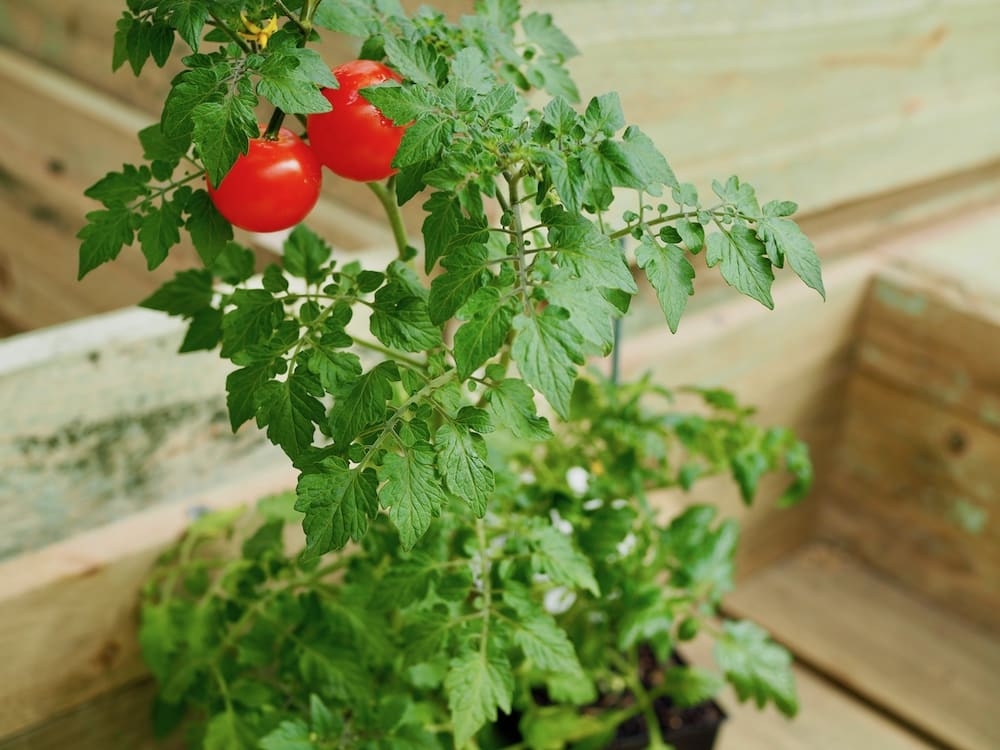
\includegraphics[width=\linewidth]{Feathergraphics/Tomato_plant.eps}
		\end{textblock*}
	
		\begin{textblock*}{30mm}(85mm,20mm)
			\includegraphics[width=\linewidth]{Feathergraphics/TYLCV_3_bush.eps}
		\end{textblock*}
	\only<2>
	{	
		\begin{textblock*}{45mm}(30mm,60mm)
			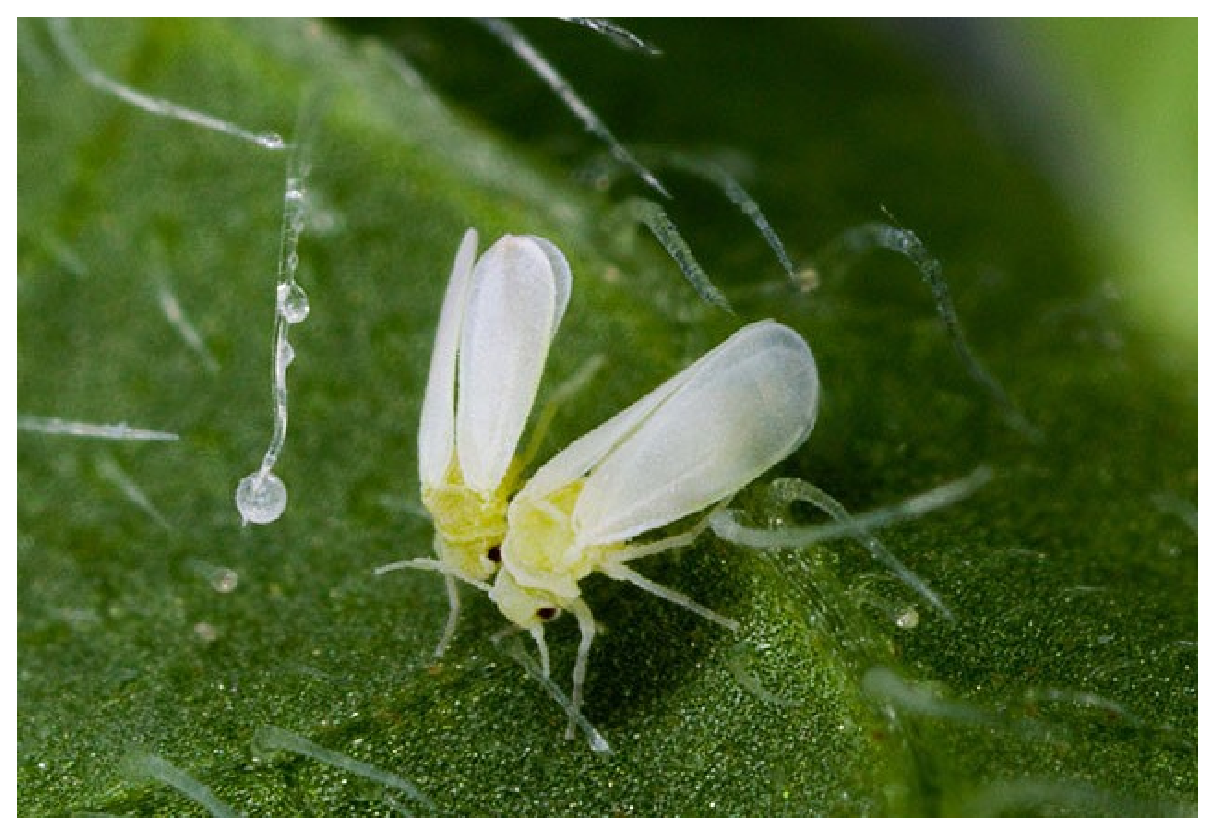
\includegraphics[width=\linewidth]{Feathergraphics/Mosca_Blanca.eps}
		\end{textblock*}
	}
\end{frame}
%%%%%%%%%%%%%%%%%%%%%%%%%%%%%%%%%%%%%%%%%%%%%%%%%%%%%%%%%%%%%%%%%%%%%%%%%%%%%%%	
\begin{frame}
		\begin{textblock*}{45mm}(10mm,25mm)
					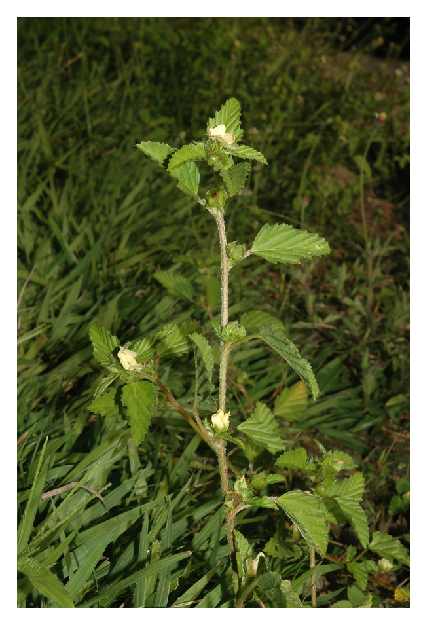
\includegraphics[width=\linewidth]{Feathergraphics/Malvastrum_coromancalianum_L.eps}
		\end{textblock*}
		\begin{textblock*}{50mm}(65mm,25mm)
					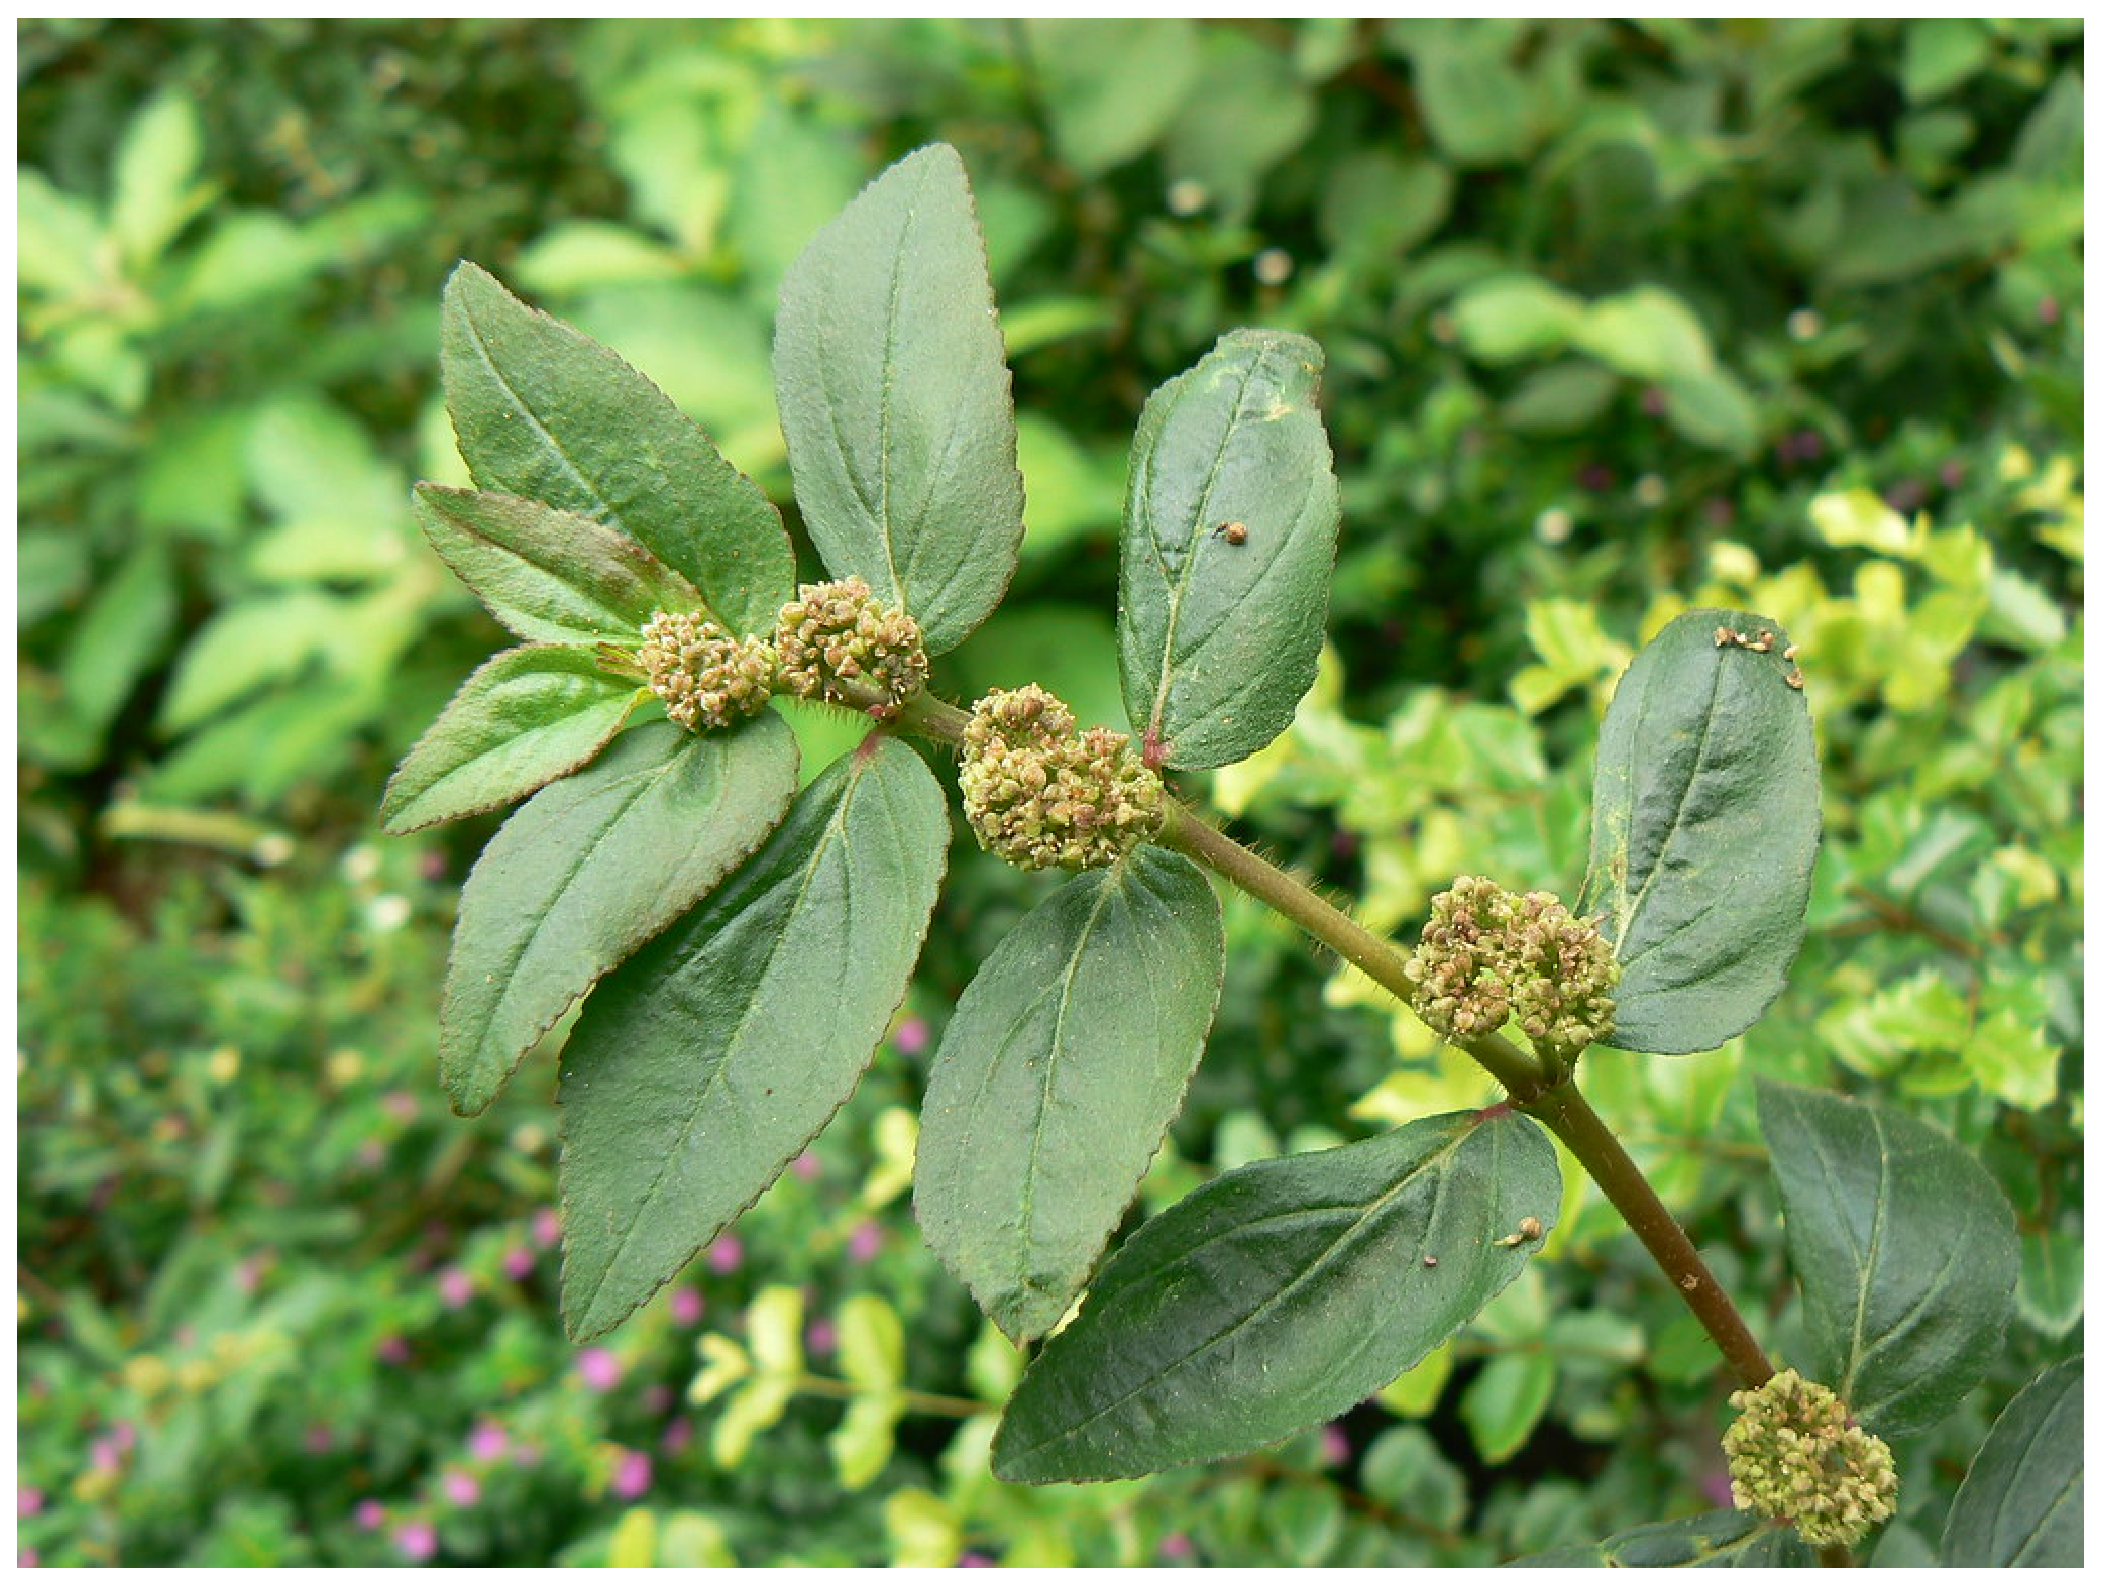
\includegraphics[width=\linewidth]{Feathergraphics/Euphorbia_geniculata_Ort.eps}
		\end{textblock*}	
\end{frame}
%%%%%%%%%%%%%%%%%%%%%%%%%%%%%%%%%%%%%%%%%%%%%%%%%%%%%%%%%%%%%%%%%%%%%%%%%%%%%%%%
%%%%%%%%%%%%%%%%%%%%%%%%%%%%%%%%%%%%%%%%%%%%%%%%%%%%%%%%%%%%%%%%%%%%%%%%%%%%%%%%
\section{Objetive}

%%%%%%%%%%%%%%%%%%%%%%%%%%%%%%%%%%%%%%%%%%%%%%%%%%%%%%%%%%%%%%%%%%%%%%%%%%%%%%%%
	\begin{frame}{}
		\begin{block}{Objetive}
			Model $\mathbf{\textcolor{greenstrong}{optimal\, phytosanitary\, policies}}$ for diseases in farm crops using ODE, PDE, SDE.
		\end{block}
	\end{frame}
%%%%%%%%%%%%%%%%%%%%%%%%%%%%%%%%%%%%%%%%%%%%%%%%%%%%%%%%%%%%%%%%%%%%%%%%%%%%%%%%
%%%%%%%%%%%%%%%%%%%%%%%%%%%%%%%%%%%%%%%%%%%%%%%%%%%%%%%%%%%%%%%%%%%%%%%%%%%%%%%%
\section{Epidemical Model}

%%%%%%%%%%%%%%%%%%%%%%%%%%%%%%%%%%%%%%%%%%%%%%%%%%%%%%%%%%%%%%%%%%%%%%%%%%%%%%%

\begin{frame}{}
	\begin{bibunit}[abbrv]
		\nocite{Holt1999b}
		\putbib
	\end{bibunit}
\end{frame}

%%%%%%%%%%%%%%%%%%%%%%%%%%%%%%%%%%%%%%%%%%%%%%%%%%%%%%%%%%%%%%%%%%%%%%%%%%%%%%%	
\begin{frame}{Plant Model without control}{Tomato Leaf Curl Virus Disease Using an Epidemiological Model}
		\begin{textblock*}{60mm}(65mm,25mm)
			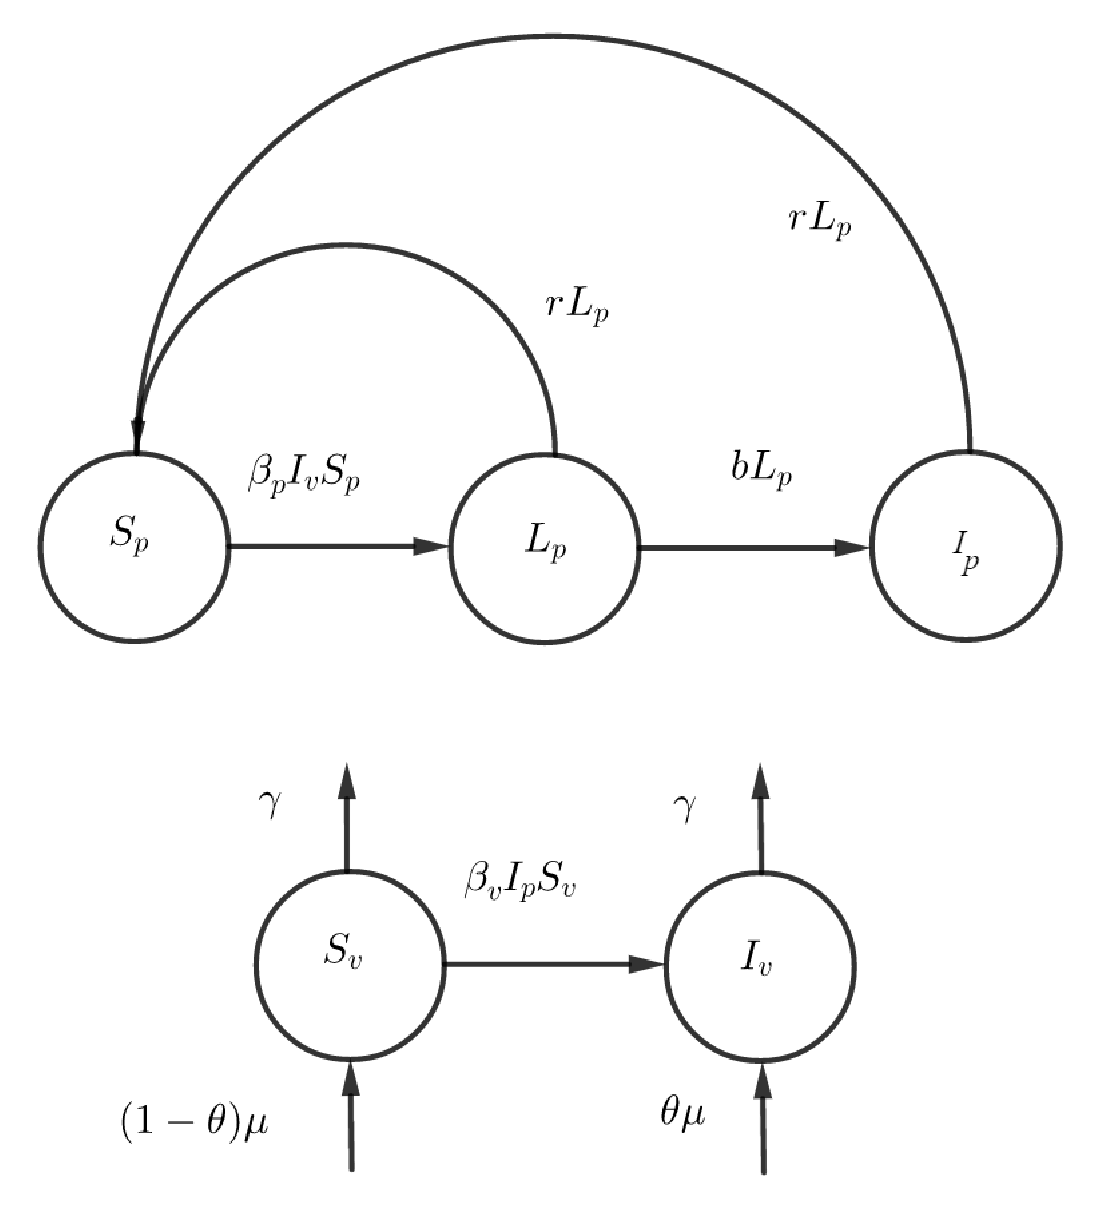
\includegraphics[width=\linewidth]{Feathergraphics/plant_diagram.eps}
		\end{textblock*}
		\begin{textblock*}{60mm}(2mm,25mm)
			\begin{graybox}{Hypothesis:}
				
				\begin{itemize}
					\item<1-> Remove from latent and infected plants,
					\item<2-> plants become latent by infected vectors,
					\item<3-> latent plants become infectious plants,
					\item<4-> vectors become infected by infected plants,
					\item<5-> vectors die or depart per day,
					\item<6-> immigration from alternative hosts.
				\end{itemize}
			\end{graybox}	
		\end{textblock*}
\end{frame}

%%%%%%%%%%%%%%%%%%%%%%%%%%%%%%%%%%%%%%%%%%%%%%%%%%%%%%%%%%%%%%%%%%%%%%%%%%%%%%%%
\subsection{Model without control}
	\begin{frame}[plain]
		\begin{textblock*}{61mm}(1mm,5mm)
			\begin{greenbox}{}
				\begin{align*}
				\frac{dS_p}{dt} &=
				-\beta_p S_p I_v +\textcolor{capri}{r}(L_p +  I_p),\\
				\frac{dL_p}{dt} &= 
				\beta_p S_p I_v -b L_p-\textcolor{capri}{r} L_p,\\
				\frac{dI_p}{dt} &=
			 b L_p - \textcolor{capri}{r} I_p,\\
				\frac{dS_v}{dt} &=
				-\beta_v S_v I_p - \textcolor{cadmiumorange}{\gamma} S_v   +(1-\theta)\mu,\\
				\frac{dI_v}{dt} &=
				\beta_v S_v I_p -\textcolor{cadmiumorange}{\gamma} I_v	+\theta\mu,\\
				S_p(0) &= S_{p_0}, L_p(0) = L_{p_0}, I_p(0) = I_{p_0},\\
				S_v(0) &= S_{v_0}, I_v(0) = I_{v_0}.
				\end{align*}
			\end{greenbox}
		\end{textblock*}
		\only<1>{
			\begin{textblock*}{50mm}(63mm,5mm)
				\begin{tabular}{|c |c |l |} 
					\hline
					Par. & Unit & Descrip. \\ [0.5ex] 
					\hline
					$\beta_p$ & vector$^{-1}$day$^{-1}$ & plants became
						\\
							&&latently infected 
						\\
							&&rate \\ 
					\hline
					$r$ & day$^{-1}$ &  replanting rate \\
					\hline
					$b$ & day$^{-1}$ & latent class
						\\ 
							&&to the infectious
						\\
							&&class rate\\
					\hline
					$\gamma$ & day$^{-1}$ & vector die
					\\ 
						&&or depart rate  \\
					\hline
					$\mu$ & plant$^{-1}$day$^{-1}$ & immigration rate \\
					\hline
					$\theta$ & proportion & proportion of
					\\
					 	&&infected vector
					\\
					 	&&arrival to crop  \\
					\hline
					$\beta_v$ & plant$^{-1}$day$^{-1}$ & vector infectious
					\\
						&&acquisition rate\\ 
					\hline
				\end{tabular}
			\end{textblock*}
		}
		\only<2>
		{
			\begin{textblock*}{55mm}(70mm,20mm)
				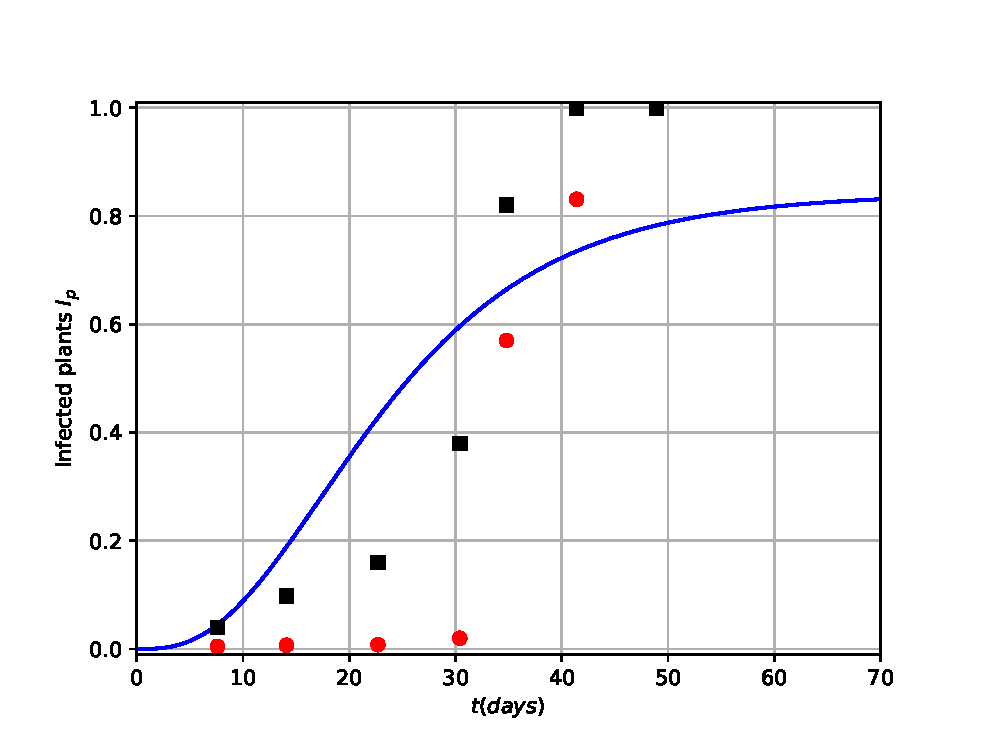
\includegraphics[width=\linewidth]{Feathergraphics/Simulation_data.eps}
			\end{textblock*}
		}
	\end{frame}
%%%%%%%%%%%%%%%%%%%%%%%%%%%%%%%%%%%%%%%%%%%%%%%%%%%%%%%%%%%%%%%%%%%%%%%%%%%%%%%%
	\begin{frame}
	
			\begin{textblock*}{50mm}(5mm,15mm)	
				\only<1,2,3>
				{
				\begin{greenbox}{}
					\begin{equation*}
					R_0=\sqrt{\frac{\beta_v\mu b\beta_p}{r^2(r+b)\gamma}}.
					\end{equation*}
				\end{greenbox}
				}
			\only<2>
			{	
				\begin{textblock*}{70mm}(5mm,45mm)
					\begin{yellowbox}{}
					
						If $R_0<1,$
						\begin{equation*}
						\lim\limits_{t\rightarrow \infty}(S_p,L_p,I_p,S_v,I_v)=(N_p,0,0,\frac{\mu}{\gamma},0).
						\end{equation*}
					\end{yellowbox}
				\end{textblock*}
			}
				\only<3>
				{
				\begin{textblock*}{70mm}(5mm,45mm)
					\begin{yellowbox}{}
					If $R_0>1,$
						\begin{equation*}
							\lim\limits_{t\rightarrow \infty}(S_p,L_p,I_p,S_v,I_v)=(S_p^*,L_p^*,I_p^*,S_v^*,I_v^*).
						\end{equation*}
				
					\end{yellowbox}
				\end{textblock*}
				}
			
		\end{textblock*}
		\begin{textblock*}{50mm}(77mm,35mm)
			\only<2>
			{
				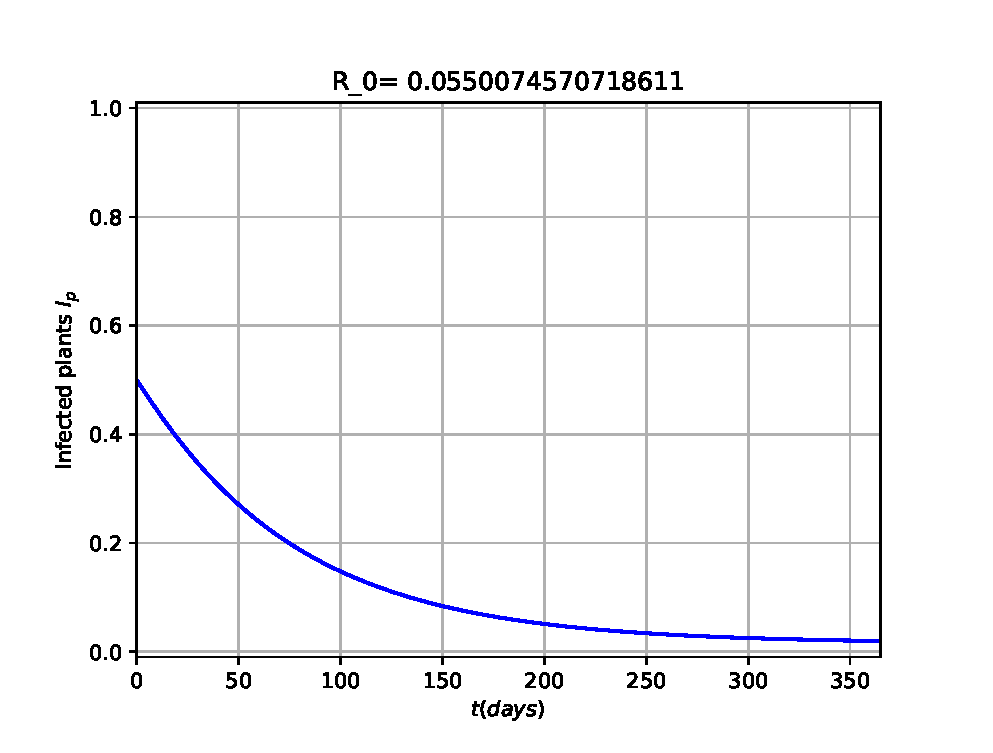
\includegraphics[width=\linewidth]{Feathergraphics/Tomato_simulation_1.eps}
			}
			\only<3>
			{
				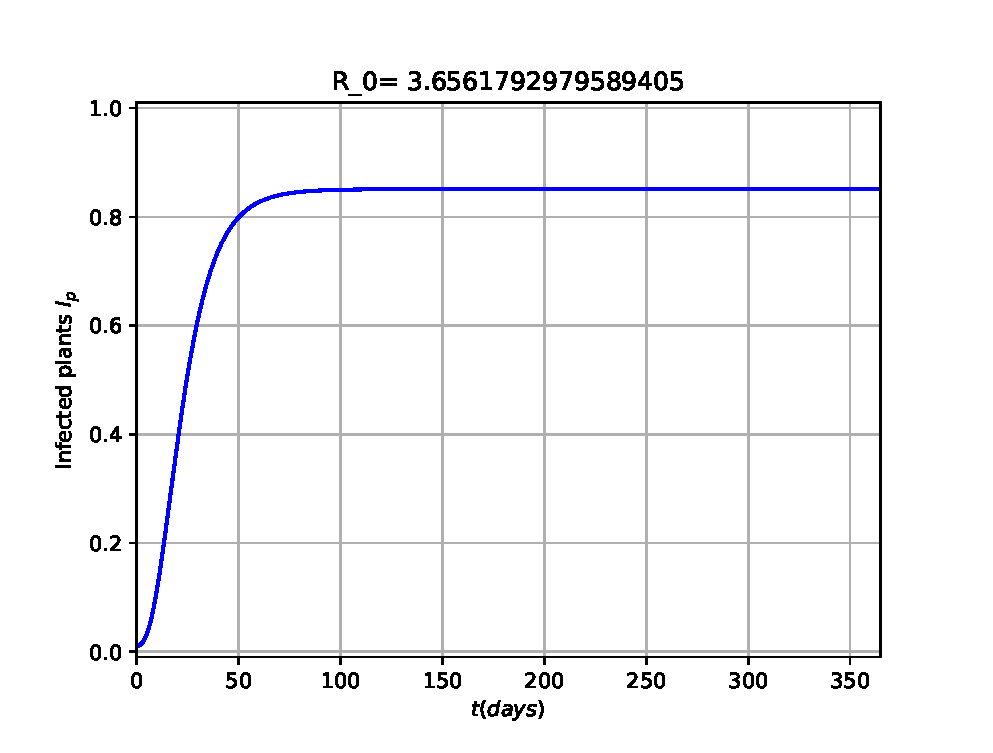
\includegraphics[width=\linewidth]{Feathergraphics/Tomato_simulation_2.eps}
			}
		\end{textblock*}	
	\end{frame}
%%%%%%%%%%%%%%%%%%%%%%%%%%%%%%%%%%%%%%%%%%%%%%%%%%%%%%%%%%%%%%%%%%%%%%%%%%%%%%%%
\subsection{Controlled Model}

	\begin{frame}[plain]%{Plant Model with control}{Tomato Leaf Curl Virus Disease Using an Epidemiological Model}
		\only<1,2,3>
		{
			\begin{textblock*}{70mm}(1mm,5mm)
				\begin{greenbox}{}
					\begin{align*}
						\frac{dS_p}{dt} &=
						-\beta_p S_p I_v +(\textcolor{capri}{r +u_1})L_p + (\textcolor{capri}{r + u_2}) I_p,\\
						\frac{dL_p}{dt} &=
						\beta_p S_p I_v -b L_p -(\textcolor{capri}{r + u_1})L_p,\\
						\frac{dI_p}{dt} &= 
						b L_p - (\textcolor{capri}{r + u_2}) I_p,\\
						\frac{dS_v}{dt} &=
						-\beta_v S_v I_p - (\textcolor{cadmiumorange}{\gamma+u_3}) S_v +(1-\theta)\mu,\\
						\frac{dI_v}{dt} &=
						\beta_v S_v I_p -(\textcolor{cadmiumorange}{\gamma+u_3}) I_v +\theta\mu,				
					\end{align*}
				\end{greenbox}
			\end{textblock*}
		}
		\only<2,3>
		{
			\begin{textblock*}{53mm}(73mm,10mm)
				\begin{yellowbox}{Controls:}
					\begin{itemize}
						\item $u_1$: replanting latent plant,
						\item $u_2$: replanting infected plants,
						\item $u_3$: fumigation.
					\end{itemize}
				\end{yellowbox}
			\end{textblock*}
		}
		\only<3>
		{
			\begin{textblock*}{115mm}(8mm,60mm)
				\begin{yellowbox}{Cost Functional}
					\begin{align*}
					\int_{0}^T	(A_1 I_p(t) + A_2 L_p(t) + A_3 I_v(t) + c_1 u_1(t)^2 + c_2 u_2(t)^2 + c_3 u_3(t)^2) dt,
					\end{align*}
				\end{yellowbox}
			\end{textblock*}
		}
		\end{frame}
%%%%%%%%%%%%%%%%%%%%%%%%%%%%%%%%%%%%%%%%%%%%%%%%%%%%%%%%%%%%%%%%%%%%%%%%%%%%%%%%
	\begin{frame}[plain]
		\begin{textblock*}{120mm}(2mm,0mm)
			\begin{yellowbox}{OC}
				\begin{align*}
				\min_{\bar{u}(\cdot)\in \tilde{\mathcal{U}}_{x_0}[t_0,T]}J(u_1,u_2,u_3)
				\end{align*}
				s.t.
				\begin{equation*}
					%\left\{ 
					\begin{aligned}
						\frac{dS_p}{dt} &=
						 -\beta_p S_p I_v +(r +u_1)L_p + (r + u_2) I_p,
						 \\
						\frac{dL_p}{dt} &=
						\beta_p S_p I_v -b L_p -(r + u_1)L_p,
						\\
						\frac{dI_p}{dt} &= 
						b L_p - (r + u_2) I_p,
						\\
						\frac{dS_v}{dt} &=
						-\beta_v S_v I_p - (\gamma+u_3) S_v +(1-\theta)\mu,
						\\
						\frac{dI_v}{dt} &=
						\beta_v S_v I_p -(\gamma+u_3) I_v +\theta\mu,
						\\
						&S_p(0) = S_{p_0}, L_p(0) = L_{p_0},
						\\
						&I_p(0) = I_{p_0},S_v(0) = S_{v_0}, I_v(0) = I_{v_0}.
						\\
						&u_i(t)\in[0,u_{i_{max}}]
						\end{aligned}%\right.
				\end{equation*}
			\end{yellowbox}
		\end{textblock*}
	\end{frame}
%%%%%%%%%%%%%%%%%%%%%%%%%%%%%%%%%%%%%%%%%%%%%%%%%%%%%%%%%%%%%%%%%%%%%%%%%%%%%%%%

%%%%%%%%%%%%%%%%%%%%%%%%%%%%%%%%%%%%%%%%%%%%%%%%%%%%%%%%%%%%%%%%%%%%%%%%%%%%%%%%
\section{Existence Theory}

\begin{frame}
	\frametitle{Existence Theory}
	\begin{textblock*}{70mm}(30mm,25mm)
		\begin{greenbox}{}
			$$\left\{ \begin{array}{l}
			\dot{x}(s)=f(s,u(s),x(s))\,\,s\in [t_0,T], \\
			x(t_0)=x_0,\\
			\end{array}
			\right.$$
	
			with terminal state constraint
			$$x(T;t_0,x_0,u(\cdot))\in M, M\subseteq \mathbb{R}^n.$$
			
		\end{greenbox}
	\end{textblock*}
	\begin{textblock*}{100mm}(15mm,65mm)
		\begin{yellowbox}{}
			$$J(t_0,x_0;u(\cdot))=\int_{t_0}^{T}g(s,u(s),x(s))ds+h(x(T)).$$
		\end{yellowbox}
	\end{textblock*}
\end{frame}
%%%%%%%%%%%%%%%%%%%%%%%%%%%%%%%%%%%%%%%%%%%%%%%%%%%%%%%%%%%%%%%%%%%%%%%%%%%%%%%%

\begin{frame}
	\begin{textblock*}{110mm}(10mm,20mm)
		\begin{graybox}{Problem $(OC)$}
			$(t_0,x_0)\in \mathbb{R}_{+}\times \mathbb{R}^n$ with $\tilde{\mathcal{U}}_{x_0}[t_0,T]\neq\emptyset$, find a $\bar{u}(\cdot)\in \tilde{\mathcal{U}}_{x_0}[t_0,T]$ s.t.
			
			\begin{equation*}
				J(t_0,x_0;\bar{u}(\cdot))=\inf_{u(\cdot)\in \tilde{\mathcal{U}}_{x_0}[t_0,T]} J(t_0,x_0;u(\cdot)).
			\end{equation*}
		\end{graybox}
	\end{textblock*}
\end{frame}
%%%%%%%%%%%%%%%%%%%%%%%%%%%%%%%%%%%%%%%%%%%%%%%%%%%%%%%%%%%%%%%%%%%%%%%%%%%%%%%%
\begin{frame}[plain]
	\begin{textblock*}{60mm}(5mm,5mm)
		\begin{graybox}{Hypothesis:}
			\begin{enumerate}[(\textbf{{C}}-1)]
				\item<1->
					$
						f:\mathbb{R}_{+}\times U
						\times \mathbb{R}^n\rightarrow 
						\mathbb{R}^n
					$ is measurable, satisfies a lipchitz
					 condition in $x$,
					$
						|f(t,u,0)|\leq L,\,
						 \forall\,(t,u)\in
						 \mathbb{R}_{+}\times U .
					$
				\item<2->
					$
						g:\mathbb{R}_{+}\times U\times 
						\mathbb{R}^n\rightarrow \mathbb{R},
					$ 
					$
						h:\mathbb{R}^n\rightarrow \mathbb{R}
					$ are measurable, and
					\begin{align*}
						&|g(s,u,x_1)-g(s,u,x_2)|+\\
						&|h(x_1)-h(x_2)|\\
						&\leq \omega(|x_1|\vee |x_2|,|x_1-x_2|)
					\end{align*}
					$
						\forall\, (s,u)\in \mathbb{R}_{+}
						\times U,x_1,x_2\in \mathbb{R}^n
					$.
				\item<3->
					For a.a. $t\in[0,T]$, Cesari property holds $\forall$ $x\in \mathbb{R}^n$.
			\end{enumerate}	
		\end{graybox}
	\end{textblock*}
	\only<2>
	{
		\begin{textblock*}{50mm}(75mm,5mm)
			\begin{yellowbox}{Modulus of continuity}
				$\omega:\mathbb{R}_{+}\times\mathbb{R}_{+}\rightarrow \mathbb{R}_{+}$, increasing, $\omega(r,0)=0$ 
				${\forall r\geq 0}$.
			\end{yellowbox}
		\end{textblock*}
	}
	\only<3>
	{
		\begin{textblock*}{50mm}(75mm,20mm)
			\begin{yellowbox}{}
				$\bar{co}(\mathbf{E})$: closed convex hull of $\mathbf{E}$,
				\begin{align*}
					&\mathbf{E}(t,x)=\{(z^0,z)\in \mathbb{R}\times \mathbb{R}^n|\\
					&z^0\geq g(t,u,x),\\
					&z=f(t,u,x),\, u\in U\}.
				\end{align*}			
			\end{yellowbox}
		\end{textblock*}
	
		\begin{textblock*}{50mm}(75mm,60mm)
			\begin{yellowbox}{Cesari property}
				\begin{equation*}
				\bigcap_{\delta}\bar{co}\mathbf{E}(t,B_{\delta}(x))=\mathbf{E}(t,x)
				\end{equation*}			
			\end{yellowbox}
		\end{textblock*}
	}
\end{frame}
%%%%%%%%%%%%%%%%%%%%%%%%%%%%%%%%%%%%%%%%%%%%%%%%%%%%%%%%%%%%%%%%%%%%%%%%%%%%%%%%

\begin{frame}[plain]
	\begin{textblock*}{60mm}(5mm,5mm)
		\begin{graybox}{Hypothesis:}
			\begin{enumerate}[(\textbf{{C}}-1)]
				\item
					$
					f:\mathbb{R}_{+}\times U
					\times \mathbb{R}^n\rightarrow 
					\mathbb{R}^n
					$ is measurable, satisfies a lipchitz
					condition in $x$,
					$
					|f(t,u,0)|\leq L,\,
					\forall\,(t,u)\in
					\mathbb{R}_{+}\times U .
					$
				\item
					$
					g:\mathbb{R}_{+}\times U\times 
					\mathbb{R}^n\rightarrow \mathbb{R},
					$ 
					$
					h:\mathbb{R}^n\rightarrow \mathbb{R}
					$ are measurable, and
					\begin{align*}
					&|g(s,u,x_1)-g(s,u,x_2)|+\\
					&|h(x_1)-h(x_2)|\\
					&\leq \omega(|x_1|\vee |x_2|,|x_1-x_2|)
					\end{align*}
					$
					\forall\, (s,u)\in \mathbb{R}_{+}
					\times U,x_1,x_2\in \mathbb{R}^n
					$.
				\item
					For a.a. $t\in[0,T]$, Cesari property holds $\forall$ $x\in \mathbb{R}^n$.
			\end{enumerate}	
		\end{graybox}
	\end{textblock*}


	
	\begin{textblock*}{55mm}(70mm,15mm)
		\begin{graybox}{Existence Theorem}
			Let ($\mathbf{C}$-1)-($\mathbf{C}$-3) hold. Then problem $(OC)$ admits at least one optimal pair.
		\end{graybox}
	\end{textblock*}
\end{frame}

%%%%%%%%%%%%%%%%%%%%%%%%%%%%%%%%%%%%%%%%%%%%%%%%%%%%%%%%%%%%%%%%%%%%%%%%%%%%%%%%

%%%%%%%%%%%%%%%%%%%%%%%%%%%%%%%%%%%%%%%%%%%%%%%%%%%%%%%%%%%%%%%%%%%%%%%%%%%%%%%%
\section{Optimal Control Characterization}

\begin{frame}[plain]
\frametitle{Optimal Control Characterization}
\begin{textblock*}{120mm}(5mm,20mm)
	\begin{yellowbox}{}
		$$\left\{ \begin{array}{l}
		\dot{x}(s)=f(s,u(s),x(s))\,\,s\in [t_0,T], \\
		x(t_0)=x_0,\\
		\end{array}
		\right.$$			
		$$J(t_0,x_0;u(\cdot))=\int_{t_0}^{T}g(s,u(s),x(s))ds+h(x(T)).$$
	\end{yellowbox}
\end{textblock*}

	\begin{textblock*}{75mm}(5mm,50mm)
		\begin{greenbox}{Hamiltonian:}
			\begin{equation*}
			H=g(t,x(t),u(t))+\langle \lambda(t),f(t,x(t),u(t))\rangle,
			\end{equation*}
		\end{greenbox}
	\end{textblock*}
\end{frame}
%%%%%%%%%%%%%%%%%%%%%%%%%%%%%%%%%%%%%%%%%%%%%%%%%%%%%%%%%%%%%%%%%%%%%%%%%%%%%%%%
\begin{frame}[plain]
	\begin{textblock*}{100mm}(15mm,15mm)
		\begin{graybox}{Additional hypothesis:}
			\begin{enumerate}[(\textbf{{C}}-4)]
				\item
				$$
					x \mapsto (f(t,u,x),g(t,u,x),h(x))
				$$
				is differentiable,
				$$
				(u,x) \mapsto (f(t,u,x),f_x(t,u,x),g(t,u,x),g_x(t,u,x),h_x(x))
				$$
				is continuous.				
			\end{enumerate}	
		\end{graybox}
	\end{textblock*}
\end{frame}
%%%%%%%%%%%%%%%%%%%%%%%%%%%%%%%%%%%%%%%%%%%%%%%%%%%%%%%%%%%%%%%%%%%%%%%%%%%%%%%%
\begin{frame}[plain]\frametitle{Optimal control characterization}
	\begin{textblock*}{120mm}(5mm,7mm)
		\begin{graybox}{Pontryagin’s Maximum Principle}
			Let ($\mathbf{C}$-1)-($\mathbf{C}$-4) hold. If $\bar{u}(t)$ and $\bar{x}(t)$ are optimal for the problem $(OC)$, then there exists a piecewise differentiable adjoint variable $\lambda(t)$ s.t.
				\begin{equation*}
					 H(t,\bar{x}(t),\bar{u}(t),\lambda(t))=\min_{u(\cdot)\in \mathcal{U}_{x_0}[t_0,T]}H(t,\bar{x}(t),u(t),\lambda(t))
				\end{equation*}
			$\forall$ $u$ at $t$,

				\begin{align*}
					\lambda'(t) &= -\frac{\partial H(t,\bar{x}(t),\bar{u}(t),\lambda(t))}{\partial x},\\
					\lambda(T) &= 0.
				\end{align*}
				\tcblower
					$$\frac{\partial H}{\partial u_i}(t,\bar{x},\bar{u})=0.$$
		\end{graybox}
		
	\end{textblock*}
		\begin{textblock*}{75mm}(5mm,79mm)
		\begin{yellowbox}{}
			\begin{equation*}
			H=g(t,x(t),u(t))+\langle \lambda(t),f(t,x(t),u(t))\rangle,
			\end{equation*}
		\end{yellowbox}
	\end{textblock*}

\end{frame}

%%%%%%%%%%%%%%%%%%%%%%%%%%%%%%%%%%%%%%%%%%%%%%%%%%%%%%%%%%%%%%%%%%%%%%%%%%%%%%%%
\begin{frame}[plain]
\frametitle{Example}
	\only<1,2>
	{
		\begin{textblock*}{70mm}(1mm,10mm)
			\begin{greenbox}{}
				\begin{align*}
				\frac{dS_p}{dt} &=
				-\beta_p S_p I_v +(\textcolor{capri}{r +u_1})L_p + (\textcolor{capri}{r + u_2}) I_p,\\
				\frac{dL_p}{dt} &=
				\beta_p S_p I_v -b L_p -(\textcolor{capri}{r + u_1})L_p,\\
				\frac{dI_p}{dt} &= 
				b L_p - (\textcolor{capri}{r + u_2}) I_p,\\
				\frac{dS_v}{dt} &=
				-\beta_v S_v I_p - (\textcolor{cadmiumorange}{\gamma+u_3}) S_v +(1-\theta)\mu,\\
				\frac{dI_v}{dt} &=
				\beta_v S_v I_p -(\textcolor{cadmiumorange}{\gamma+u_3}) I_v +\theta\mu,				
				\end{align*}
			\end{greenbox}
		\end{textblock*}
	}
	\only<2>
		{
			\begin{textblock*}{55mm}(72mm,10mm)
				\begin{greenbox}{}
					\begin{align*}
						H&=A_1I_v+A_2L_p+A_3I_v\\
						&+\sum_{i=1}^{3}c_iu_i^2\\
						&+\textcolor{colComments}{\lambda_1}(-\beta_p S_p I_v +(r +u_1)L_p\\
						&+ (r + u_2) I_p)\\
						&+\textcolor{colComments}{\lambda_2}(\beta_p S_p I_v -b L_p\\
						&-(r + u_1)L_p)\\
						&+\textcolor{colComments}{\lambda_3}(b L_p - (r + u_2) I_p)\\
						&+\textcolor{colComments}{\lambda_4}(-\beta_v S_v I_p - (\gamma+u_3) S_v\\ &+(1-\theta)\mu)\\
						&+\textcolor{colComments}{\lambda_5}(\beta_v S_v I_p -(\gamma+u_3) I_v\\
						& +\theta\mu).
					\end{align*}
				\end{greenbox}
			\end{textblock*}
		}
\end{frame}

%%%%%%%%%%%%%%%%%%%%%%%%%%%%%%%%%%%%%%%%%%%%%%%%%%%%%%%%%%%%%%%%%%%%%%%%%%%%%%%%

\begin{frame}[plain]
	\only<1,2,3>
	{	
		\begin{textblock*}{80mm}(25mm,1mm)
			\begin{greenbox}{}
				\begin{align*}
				\frac{d\lambda_1}{dt} &=\beta_p (\lambda_1-\lambda_2),\\
				\frac{d\lambda_2}{dt} &=-A_2+(r+u_1)(\lambda_2-\lambda_1)+b(\lambda_2-\lambda_3),\\
				\frac{d\lambda_3}{dt} &-A_1+(r+u_2)(\lambda_3-\lambda_1)+\beta_vS_v(\lambda_4-\lambda_5),\\
				\frac{d\lambda_4}{dt} &=\beta_v I_p(\lambda_4-\lambda_5)+(\gamma+u_3)\lambda_4,\\
				\frac{d\lambda_5}{dt} &=-A_3+\beta_p S_p(\lambda_1-\lambda_2)+(\gamma+u_3)\lambda_5,				
				\end{align*}
			\end{greenbox}	
		\end{textblock*}
	}
	\only<2,3>
	{
		\begin{textblock*}{32mm}(10mm,70mm)
			\begin{yellowbox}{}
				$\frac{\partial H}{\partial u}(\bar{u})=0 \Rightarrow$
			\end{yellowbox}
		\end{textblock*}
	}
	\only<3>
	{
	\begin{textblock*}{70mm}(50mm,55mm)
		\begin{yellowbox}{}
			\begin{align*}
				\bar{u}_1&=\min\left(\max\left(0,\frac{\bar{L_p}(\lambda_2-\lambda_1)}{2c_1}\right),u_1^{max}\right)\\
				\bar{u}_2&=\min\left(\max\left(0,\frac{\bar{I_p}(\lambda_3-\lambda_1)}{2c_2}\right),u_2^{max}\right)\\
				\bar{u}_3&=\min\left(\max\left(0,\frac{\bar{S_v}\lambda_4+\bar{I_v}\lambda_5}{2c_3}\right),u^{max}_i\right)
			\end{align*}
		\end{yellowbox}
	\end{textblock*}
	}
\end{frame}
%%%%%%%%%%%%%%%%%%%%%%%%%%%%%%%%%%%%%%%%%%%%%%%%%%%%%%%%%%%%%%%%%%%%%%%%%%%%%%%%

%%%%%%%%%%%%%%%%%%%%%%%%%%%%%%%%%%%%%%%%%%%%%%%%%%%%%%%%%%%%%%%%%%%%%%%%%%%%%%%%
\section{Simulations}

	\begin{frame}
		\frametitle{Case with one controls}
		\begin{figure}
			\centering	
			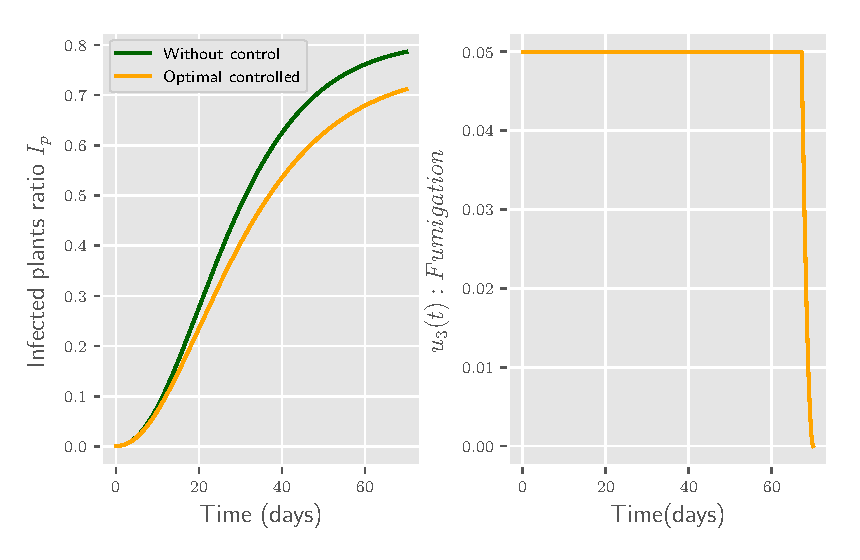
\includegraphics[scale=0.5]{Feathergraphics/figure_1_tomato_one_control.eps}
		\end{figure}	
	\end{frame}
%%%%%%%%%%%%%%%%%%%%%%%%%%%%%%%%%%%%%%%%%%%%%%%%%%%%%%%%%%%%%%%%%%%%%%%%%%%%%%%	
	\begin{frame}
		\frametitle{Case with two controls}
		\begin{figure}
			\centering	
			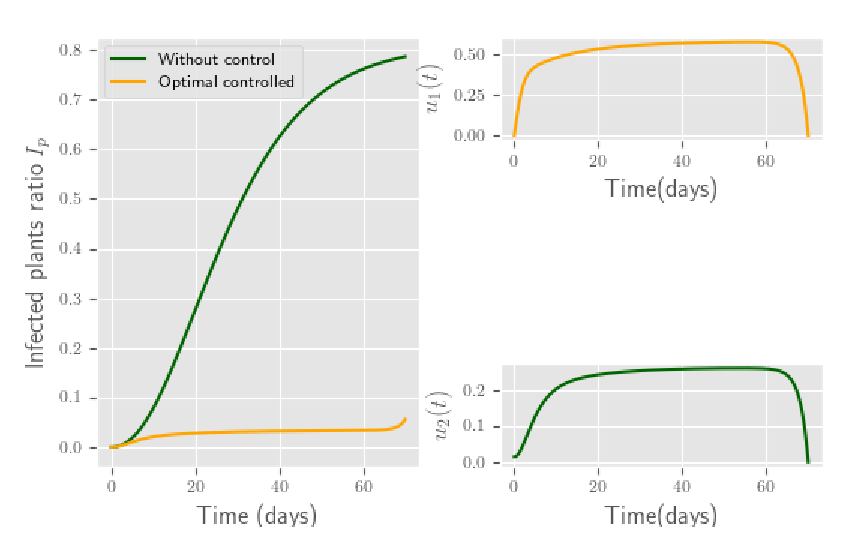
\includegraphics[scale=0.5]{Feathergraphics/two_control_simulation_2.eps}
		\end{figure}	
	\end{frame}
%%%%%%%%%%%%%%%%%%%%%%%%%%%%%%%%%%%%%%%%%%%%%%%%%%%%%%%%%%%%%%%%%%%%%%%%%%%%%%%	
	\begin{frame}
		\begin{figure}
			\frametitle{Case with three controls}
			\centering	
			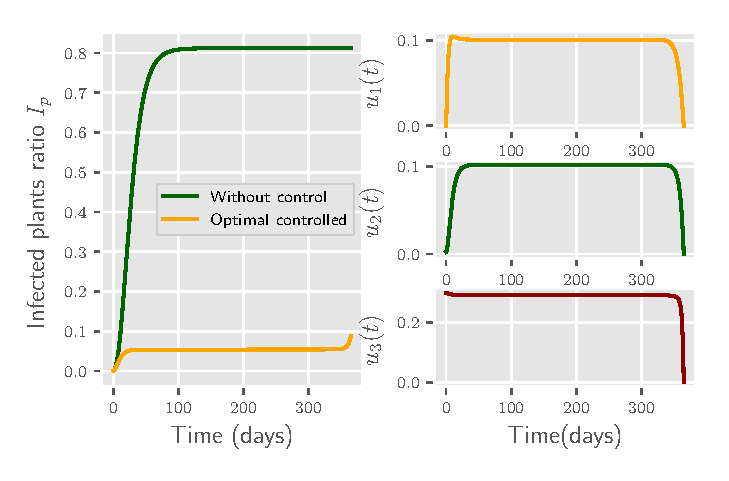
\includegraphics[scale=0.5]{Feathergraphics/three_controls_simulation_1.eps}
		\end{figure}	
	\end{frame}
%%%%%%%%%%%%%%%%%%%%%%%%%%%%%%%%%%%%%%%%%%%%%%%%%%%%%%%%%%%%%%%%%%%%%%%%%%%%%%%%

%%%%%%%%%%%%%%%%%%%%%%%%%%%%%%%%%%%%%%%%%%%%%%%%%%%%%%%%%%%%%%%%%%%%%%%%%%%%%%%%
\section{Perspective}

\begin{frame}[plain]
	\begin{center}
		{\LARGE Perspectives}
	\end{center}
\end{frame}
%%%%%%%%%%%%%%%%%%%%%%%%%%%%%%%%%%%%%%%%%%%%%%%%%%%%%%%%%%%%%%%%%%%%%%%%%%%%%%%%
\begin{frame}[plain]
	\frametitle{Stochastic optimal control theory}
	\begin{textblock*}{100mm}(15mm,10mm)
		\begin{graybox}{}
			$(\Omega,\mathscr{F},\{\mathscr{F}_t\}_{t\geq 0},\mathbb{P})$,\\ $W(t):m\text{-dimensional Brownian motion}$.
			
			\begin{align*}
				dx(t)&=
				f(t,u(t),x(t))dt+\sigma(t,u(t),x(t))dW(t)\\
				x(0)&=
				x_0,\\
				f&:
				[0,T]\times U\times\mathbb{R}^n\rightarrow\mathbb{R}^n, \sigma:[0,T]\times U\times\mathbb{R}^n\rightarrow\mathbb{R}^{n+m},\\
				U&:
				\text{separable metric space}.\\
			\end{align*}
		\end{graybox}
	\end{textblock*}

	\begin{textblock*}{100mm}(15mm,65mm)
		\begin{yellowbox}{}
			$\mathcal{U}[0,T]:=\{u:[0,T]\times\Omega\rightarrow U | u(\cdot)\,\text{is}\,\{\mathscr{F}_t\}_{t\geq 0}\text{-adapted}\}$
		\end{yellowbox}
	\end{textblock*}
\end{frame}
%%%%%%%%%%%%%%%%%%%%%%%%%%%%%%%%%%%%%%%%%%%%%%%%%%%%%%%%%%%%%%%%%%%%%%%%%%%%%%%%
\begin{frame}[plain]
	\begin{textblock*}{90mm}(20mm,15mm)
		\begin{graybox}{Weak formulation of optimal control}
			 A 6-tuple $\pi=(\Omega,\mathscr{F},\{\mathscr{F}_t\}_{t\geq 0},\mathbb{P},W(\cdot),u(\cdot))$ is a w-admissible control, $(u(\cdot),x(\cdot))$ is a w-admissible pair, if
			\begin{itemize}[<+->]
				\item $(\Omega,\mathscr{F},\{\mathscr{F}_t\}_{t\geq 0},\mathbb{P})$ is a filtered probability space satisfying the usual conditions,
				\item $W(t)$ is an $m$-dimensional standard Brownian motion defined on $(\Omega,\mathscr{F},\{\mathscr{F}_t\}_{t\geq 0},\mathbb{P})$,
				\item $u(\cdot)$ is an $\{\mathscr{F}_t\}_{t\geq 0}\text{-adapted}$ process on $(\Omega,\mathscr{F},\mathbb{P})$ taking values in $U$,
				\item $x(\cdot)$ is unique solution,
				\item some prescribed state constraints are satisfied,
				\item $g(\cdot,u(\cdot),x(\cdot))\in L^1_{\mathscr{F}}(0,T;\mathbb{R})$ and $h(x(T))\in L^1_{\mathscr{F}_T}(\Omega;\mathbb{R})$
			\end{itemize}
		\end{graybox}
	\end{textblock*}
\end{frame}
%%%%%%%%%%%%%%%%%%%%%%%%%%%%%%%%%%%%%%%%%%%%%%%%%%%%%%%%%%%%%%%%%%%%%%%%%%%%%%%%
\begin{frame}[plain]
		\begin{textblock*}{80mm}(25mm,15mm)
		\begin{yellowbox}{}
			\begin{equation*}
				J(u(\cdot))= \mathbb{E}\left\{\int_{0}^{T}g(t,u(t),x(t))dt+h(x(T))\right\}
			\end{equation*}
		\end{yellowbox}
	\end{textblock*}
	
	
	\begin{textblock*}{90mm}(20mm,40mm)
		\begin{graybox}{$(WS)$}
				\begin{equation*}
					J(\bar{\pi})=\inf_{\pi\in \mathcal{U}^w_{ad}[0,T]} J(\pi)
					\tag{*}
				\end{equation*}
				s.t.
				\begin{align*}
					dx(t)&=
					f(t,u(t),x(t))dt+\sigma(t,u(t),x(t))dW(t)\\
					x(0)&=
					x_0,
				\end{align*}
				\tcblower
					problem (WS) is finite, if r.h.s. of (*) is finite. 
			\end{graybox}
	\end{textblock*}
\end{frame}
%%%%%%%%%%%%%%%%%%%%%%%%%%%%%%%%%%%%%%%%%%%%%%%%%%%%%%%%%%%%%%%%%%%%%%%%%%%%%%%%
\begin{frame}[plain]
	\begin{textblock*}{110mm}(10mm,10mm)
		\begin{graybox}{Hypothesis:}
			\begin{enumerate}[(\textbf{{SE}}-1)]
				\item<1->
					$(U,d)$ is a compact metric space and $T>0$,
				\item<2->
					$f,\sigma,g$, and $h$ are all continous, and $\exists L>0$ s.t. $\psi(t,u,x)=\{f(t,u,x),\sigma(t,u,x),g(t,u,x),h(x)\}$, 
					
					\begin{align*}
						|\psi(t,u,x)-\psi(t,u,\hat{x})|&\leq L|x-\hat{x}|,\\
						&\forall t\in [0,T], x,\hat{x}\in \mathbb{R}^n,u\in U,\\
						|\psi(t,u,0)|&\leq L \forall (t,u)\in[0,T]\times U.
					\end{align*}  
				\item<3->
					$\forall (t,x)\in [0,T]\times \mathbb{R}^n$, the set
					\begin{align*}
						(f,\sigma\sigma^T,g)(t,x,U)&:=\{(f_i(t,u,x),(\sigma\sigma^T)^{ij}(t,u,x),g(t,u,x))|\\
						&u\in U,i=1,\ldots,n,j=1,\ldots,m\}
					\end{align*}
					is convex in $\mathbb{R}^{m+nm+1}$,
				\item<4->
					$S(t)\equiv\mathbb{R}^n$.
			\end{enumerate}	
		\end{graybox}
	\end{textblock*}
\end{frame}
%%%%%%%%%%%%%%%%%%%%%%%%%%%%%%%%%%%%%%%%%%%%%%%%%%%%%%%%%%%%%%%%%%%%%%%%%%%%%%%%
\begin{frame}[plain]
	
	\begin{textblock*}{100mm}(15mm,20mm)
		\begin{graybox}{Existence Theorem (weak formulation)}
			Under ($\mathbf{SE}$1)-($\mathbf{SE}$4), if (WS) is finite, then it admits an optimal control.
		\end{graybox}
	\end{textblock*}

\end{frame}
%%%%%%%%%%%%%%%%%%%%%%%%%%%%%%%%%%%%%%%%%%%%%%%%%%%%%%%%%%%%%%%%%%%%%%%%%%%%%%%%
\begin{frame}[plain]
%hamilton jacobi velma y una paso intermedio es resolver la ecuación de viscosidad

\begin{bibunit}[abbrv]
	\nocite{Lions1971}
	\putbib
\end{bibunit}
	\begin{bibunit}[abbrv]
		\nocite{Wendell2006}
		\putbib
	\end{bibunit}
	\begin{bibunit}[abbrv]
		\nocite{Fredi2010}
		\putbib
	\end{bibunit}
\end{frame}

%%%%%%%%%%%%%%%%%%%%%%%%%%%%%%%%%%%%%%%%%%%%%%%%%%%%%%%%%%%%%%%%%%%%%%%%%%%%%%%%

%%%%%%%%%%%%%%%%%%%%%%%%%%%%%%%%%%%%%%%%%%%%%%%%%%%%%%%%%%%%%%%%%%%%%%%%%%%%%%%%


%%%%%%%%%%%%%%%%%%%%%%%%%%%%%%%%%%%%%%%%%%%%%%%%%%%%%%%%%%%%%%%%%%%%%%%%%%%%%%%%

\begin{frame}{Bibliography}
	\begin{bibunit}[abbrv]
		\nocite{Bokil2019optimal}
		\putbib
	\end{bibunit}

	\begin{bibunit}[abbrv]
		\nocite{Grandits2019}
		\putbib
	\end{bibunit}

	\begin{bibunit}[abbrv]
		\nocite{yong1999stochastic}
		\putbib
	\end{bibunit}

\end{frame}
%%%%%%%%%%%%%%%%%%%%%%%%%%%%%%%%%%%%%%%%%%%%%%%%%%%%%%%%%%%%%%%%%%%%%%%%%%%%%%%%
%%%%%%%%%%%%%%%%%%%%%%%%%%%%%%%%%%%%%%%%%%%%%%%%%%%%%%%%%%%%%%%%%%%%%%%%%%%%%%%%
\end{document}